\documentclass[twoside]{article}
\usepackage[a4paper]{geometry}
\geometry{verbose,tmargin=2.5cm,bmargin=2cm,lmargin=2cm,rmargin=2cm}
\usepackage{fancyhdr}
\pagestyle{fancy}

% nastavení pisma a~češtiny
\usepackage{lmodern}
\usepackage[T1]{fontenc}
\usepackage[utf8]{inputenc}
\usepackage[czech]{babel}

% odkazy
\usepackage{url}

\usepackage{float}
% vícesloupcové tabulky
\usepackage{multirow}
\usepackage{listings}
\usepackage{xcolor}
\usepackage{amssymb}
\usepackage{gensymb}
\usepackage{bbold}
\usepackage{amsmath}
\usepackage{siunitx}
\usepackage{mathtools}
\usepackage{commath}

% vnořené popisky obrázků
\usepackage{subcaption}

% automatická konverze EPS 
\usepackage{graphicx} 
\usepackage{epstopdf}
\epstopdfsetup{update}

\graphicspath{{./images}}

% odkazy a~záložky
\usepackage[unicode=true, bookmarks=true,bookmarksnumbered=true,
bookmarksopen=false, breaklinks=false,pdfborder={0 0 0},
pdfpagemode=UseNone,backref=false,colorlinks=true] {hyperref}


% Poznámky při překladu
\usepackage{xkeyval}	% Inline todonotes
\usepackage[textsize = footnotesize]{todonotes}
\presetkeys{todonotes}{inline}{}

%https://tex.stackexchange.com/questions/2783/bold-calligraphic-typeface
\DeclareMathAlphabet\mathbfcal{OMS}{cmsy}{b}{n}

% enumerate zacina s pismenem
\renewcommand{\theenumi}{\alph{enumi}}

% smaz aktualni page layout
\fancyhf{}
% zahlavi
\usepackage{titling}
\fancyhf[HC]{\thetitle}
\fancyhf[HLE,HRO]{\theauthor}
\fancyhf[HRE,HLO]{\today}
 %zapati
\fancyhf[FLE,FRO]{\thepage}

% údaje o autorovi
\title{VSY - SW UART - dokumentace}
\author{Vojtěch Michal}
\date{\today}

%customize code listing
\definecolor{codegreen}{rgb}{0,0.6,0}
\definecolor{codegray}{rgb}{0.5,0.5,0.5}
\definecolor{codepurple}{rgb}{0.58,0,0.82}
\definecolor{backcolour}{rgb}{0.95,0.95,0.92}

\lstdefinestyle{mystyle}{
    backgroundcolor=\color{backcolour},   
    commentstyle=\color{codegreen},
    keywordstyle=\color{magenta},
    numberstyle=\tiny\color{codegray},
    stringstyle=\color{codepurple},
    basicstyle=\ttfamily\footnotesize,
    breakatwhitespace=false,         
    breaklines=true,                 
    captionpos=b,                    
    keepspaces=true,                 
    numbers=left,                    
    numbersep=5pt,                  
    showspaces=false,                
    showstringspaces=false,
    showtabs=false,                  
    tabsize=2
}

\lstset{style=mystyle}

\begin{document}

\maketitle

Cílem úlohy je emulovat softwarově přenos dat přes UART. Periodicky je vysílána dvoubajtová zpráva s iniciálami mého jména -- znaky "VM".
Mezi dvěma zprávami je interval rovný dvojonásobku délky zprávy, kdy jsou signály v recesivní úrovni.

\section{Parametry komunikace}
Použitý baudrate $f_{baud} = 9600$ baud, 1 stop bit, bez parity. Vysílací pin je v konfiguraci ouput push-pull (pozor na konflikty při připojení jiného obvodu).
V době mezi zprávami je signál držen standardně v logické jedničce (3V3), bajty se přenáší standardně od nejméně významného bitu.

\begin{table}[htbp]
    \centering
    \begin{tabular}{c|c}
        Parametr & Hodnota \\ \hline
        Délka bitu $T_{bit}$ & $ f_{baud}^{-1} = 104~\mu\text{s}$ \\
        délka \textit{SYNC\_PULSE} $T_{sync}$ & $\frac{T_{bit}}{4} = 26~\mu\text{s}$ \\
        délka zprávy v bitech $N$ & $(1+8+1) \cdot 2 = 20$ bit \\ 
        délka zprávy $T_{message}$&$N\cdot T_{bit} = 2,08 \text{ ms}$ \\
        interval mezi zprávami $T_{pause}$&$2\cdot T_{message} = 4,16 \text{ ms}$.
    \end{tabular}
    \caption{Časování použité v komunikaci}
    \label{table:casovani}
\end{table}


\section{Pinout}
Použité piny jsou uvedené v tabulce \ref{table:pinout}.
Na pinu \textit{UART\_DATA} jsou vysílány bity zprávy. Na pinu \textit{SYNC\_PULSE} je vždy uprostřed periody bitu vyslán krátký puls (dlouhý jednu čtvrtinu
délky bitu, trvá od 50 \% bitu do 75 \% bitu). Tento puls umožňuje synchonizaci přijímače, náběžná hrana označuje doporučený sample point, kdy jsou přenášená data stabilní.


\begin{table}[htbp]
    \centering
    \begin{tabular}{c|c|c}
        pin MCU & PA5 & PA6 \\ \hline
        pin Nuclea & D13 & D12 \\ \hline
        signál & UART\_DATA & SYNC\_PULSE
    \end{tabular}
    \caption{Piny využívané aplikací}
    \label{table:pinout}
\end{table}

\section{Časové průběhy}

Analýza časových průběhů byla provedena s pomocí programu EMBO \cite{EMBO}. Na všech násleudjících obrázcích
je kanál 1 (modrý) připojen na \textit{USART\_DATA} a kanál 2 (červený) připojen na \textit{SYNC\_PULSE}.

Na obrázku \ref{fig:zprava} je zachycena celá zpráva, jak ji MCU vysílá na pinu \textit{UART\_DATA}.
Na obrázku \ref{fig:timing} jsou poté s pomocí horizontálních kurzorů přiblíženy časové parametry komunikace.
Je ukázáno, že perioda signálů je skutečně $\frac{1}{9600}$ sekund a že \textit{SYNC\_PULSE} je dlouhý čtvrtinu
periody.
Na obrázku \ref{fig:decoded} je poté přenášená zpráva dekódována na logické úrovně, binární i hexadecimání hodnotu přenášených bajtů
a konečně na přenášené znaky pomocí jejich ASCII hodnot. Systém skutečně přenáší dvojici znaků \textbf{VM}.
Na obrázku \ref{fig:prodleva} je časová osa prodloužena a je tak možno zachytit více zpráv. Je zdůrazněn interval mezi dvěma přenosy.

\begin{figure}[htbp]
    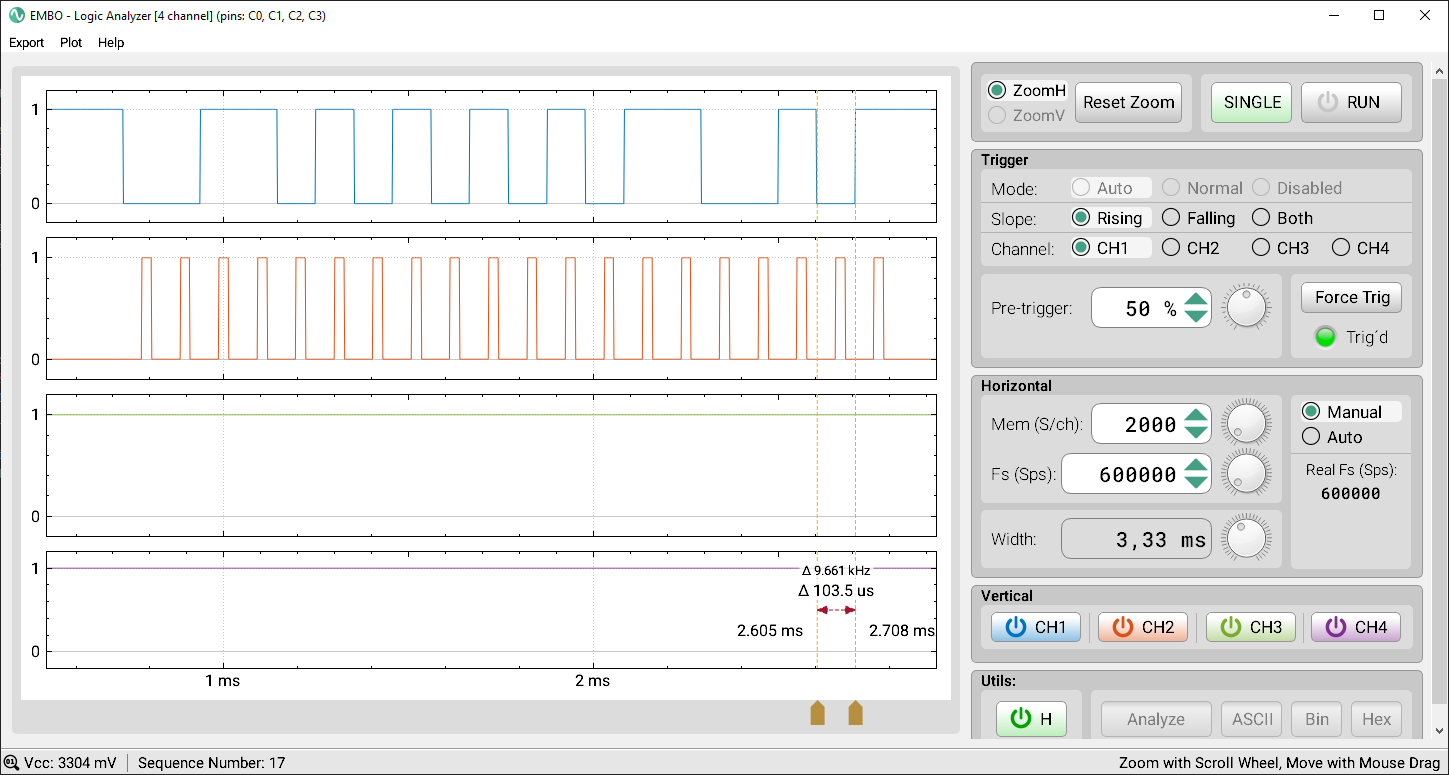
\includegraphics[width=\linewidth]{embo_zprava.png}
    \caption{Přenášená zpráva zachycená na logickém analyzátoru}
    \label{fig:zprava}
\end{figure}

\begin{figure}[htbp]
    \centering % <-- added
\begin{subfigure}{0.45\textwidth}
  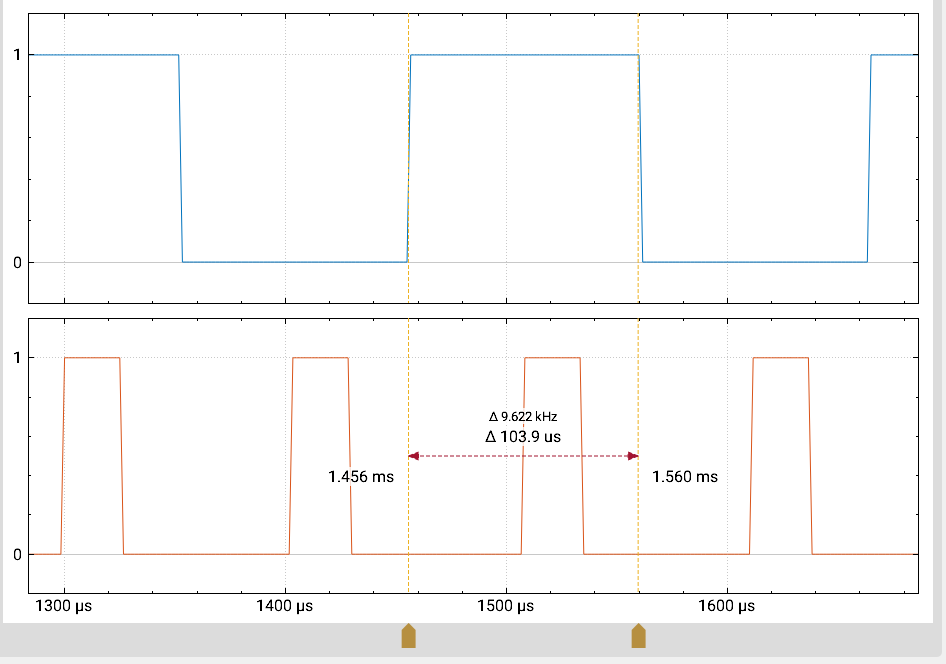
\includegraphics[width=\linewidth]{bit_detail.png}
  \caption{Časování signálu \textit{UART\_DATA}}
\end{subfigure}\hfil % <-- added
\begin{subfigure}{0.45\textwidth}
	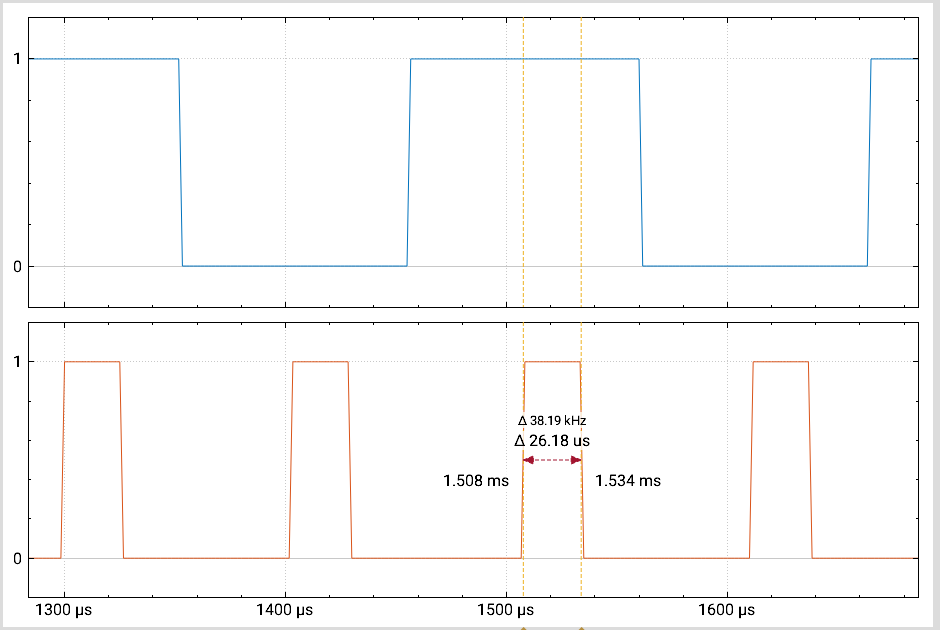
\includegraphics[width=\linewidth]{sync_detail.png}
	\caption{Časování signálu \textit{SYNC\_PULSE}}
\end{subfigure}
\caption{Časové parametry komunikace}
\label{fig:timing}
\end{figure}

\begin{figure}[htbp]
    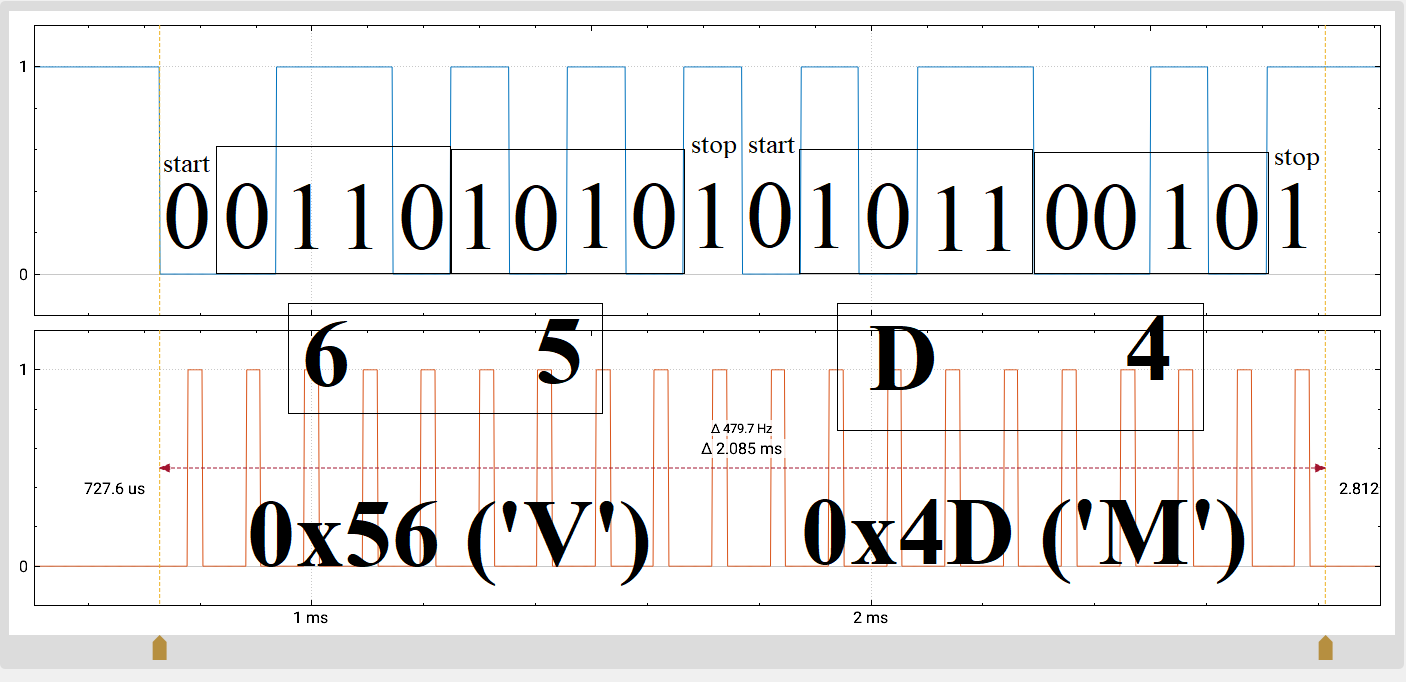
\includegraphics[width=\linewidth]{decoded.png}
    \caption{Dekódovaná zpráva}
    \label{fig:decoded}
\end{figure}

\begin{figure}[htbp]
    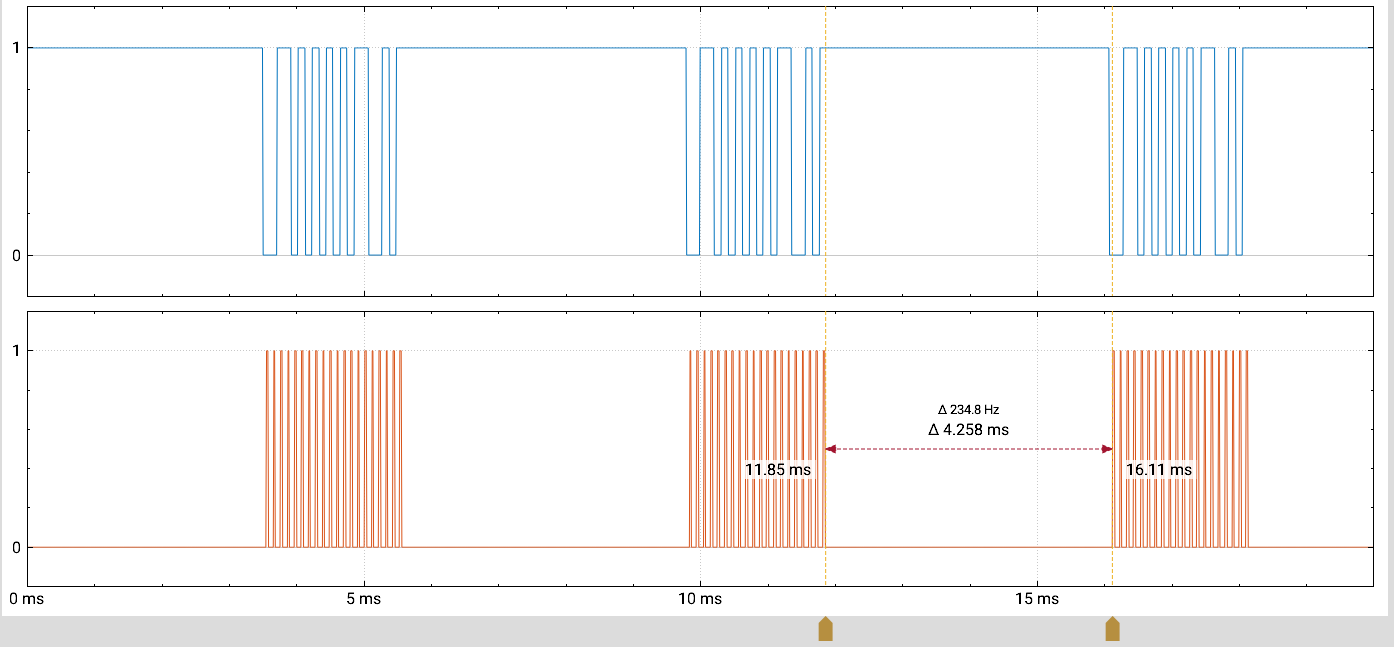
\includegraphics[width=\linewidth]{vic_zprav.png}
    \caption{Prodleva mezi dvěma po sobě jdoucími zprávami}
    \label{fig:prodleva}
\end{figure}

\begin{thebibliography}{9}
    
    \bibitem{EMBO}
    EMBO (Embedded Oscilloscope), Ing. Jakub Pařez, \url{https://embedded.fel.cvut.cz/platformy/embo}
\end{thebibliography}


\end{document}